\makeatletter
\def\input@path{{../../}}
\makeatother
\documentclass[../../main.tex]{subfiles}

\graphicspath{
	{../../img/}
	{../img/}
	{img/}
}

\begin{document}
\section{Поточечная и равномерная сходимость рядов и последовательностей ФКП}

Рассмотрим последовательность $ \phi_n,\, n \in \N $~--- ФКП, определенную для 
односвязной области $ z \in D $.

$ \phi_n(z) $ сходится поточечно к $ f(z),\ z \in D $, если

\begin{equation}\label{34:1}
	\forall \eps > 0 \quad \forall z \in D \quad \exists\nu = \nu_\eps (z) 
	\in \R\, :\,
	\forall n \geq \nu \implies |\phi_n(z) - f(z)| \leq \eps.
\end{equation}
\[ \eqref{34:1} \implies \exists \underset{n \to \infty}{\lim} \phi_n (z) 
= f(z),\ 
\forall z \in D \qquad \phi_n(z) \overset{D}{\underset{n \to 
\infty}\longrightarrow} f(z). \]

Последовательность $ (\phi_n(z)) $ называется равномерно сходящейся к $ f(z) 
$, если
\begin{equation}\label{34:2}
	\forall \eps > 0 \quad \exists\nu_\eps \in \R\, :\,
	\forall n \geq \nu,\, \forall z \in D \implies |\phi_n(z) - f(z)| \leq \eps.
\end{equation}

$ \eqref{34:2} $ записывают следующим образом:
\[ \phi_n(z) \overset{D}{\underset{n \to \infty}\rightrightarrows} f(z). \]

Нетрудно видеть, что из $ \eqref{34:2} \implies \eqref{34:1} $. Обратное, 
вообще говоря, неверно.

Здесь, как и в действительном случае, справедливы следующие теоремы.

\begin{thm}[cупремальный критерий равномерной сходимости ФП~КП]
	\[ \phi_n(z) \overset{D}{\underset{n \to \infty}\rightrightarrows} f(z) \iff 
	\underset{z \in D}{\sup}|\phi_n(z) - f(z)| \appr{n \rightarrow \infty} 0 \]
\end{thm}

\begin{thm}[мажорантный признак равномерной сходимости ФП~КП]
	Если 
	\[ \exists a_n \geq 0 \in \R :\, |\phi_n(z) - f(z)| \leq a_n,\ \forall n 
	\in \N,\ \forall z \in D, \]
	и если $ a_n \appr{n \rightarrow \infty} 0, $
	то $ \phi_n(z) \overset{D}{\underset{n \to \infty}\rightrightarrows} f(z) $.
\end{thm}

\begin{thm}[достаточное условие неравномерной сходимости]
	Если
	\[ \exists (z_n) \in D\, :\, |\phi_n(z_n) - f(z_n)| \underset{n \to 
	\infty}{\not \rightarrow} 0, \]
	то
	$ \phi_n(z) \overset{D}{\underset{n \to \infty}{\not \rightrightarrows}} 
	f(z) $.
\end{thm}

Обобщаются на комплексные ФП также следующие результаты равномерной 
сходимости действительных ФП: теорема Стокса-Зейделя, предельный переход, 
дифференцирование и интегрирование.

Для ФР $ \sum\limits_{n = 1}^{\infty} u_n(z) = u_1(z) + \ldots + u_n(z) + 
\dots,\ z \in D $
поточечная и равномерная сходимость определяется через соответствующую 
сходимость последовательности частных сумм $ S_n(z) = \sum\limits_{k = 1}^{n} 
u_k(z): $

\begin{enumerate}
	\item $ \sum\limits_{n = 1}^{\infty} u_n(z) \overset{D}{\longrightarrow} S(z) 
	\iff S_n(z) \overset{D}{\underset{n \to \infty}\longrightarrow} S(z) $,
	
	\item $ \sum\limits_{n = 1}^{\infty} u_n(z) \overset{D}\rightrightarrows S(z) 
	\iff S_n(z) \overset{D}{\underset{n \to \infty}\rightrightarrows} S(z) $.
\end{enumerate}

Здесь также справедлива следующая теорема:

\begin{thm}[мажорантный признак Вейерштрасса для ФР~КП]
	Если
	\[ \exists a_n \geq 0 : |u_n(z)| \leq a_n\quad \forall n \in \N \quad \forall 
	z \in D, \]
	то в случае, когда $ \sum\limits_{n = 1}^{\infty} a_n $ сходится, ряд $ 
	\sum\limits_{n = 1}^{\infty} u_n(z) \overset{D}\rightrightarrows $.
\end{thm}

По аналогии с действительным случаем доказывается теорема Стокса-Зейделя 
непрерывности суммы ФР~КП.

\begin{thm}[Стокса-Зейделя]
Если $ \forall u_n (z) $ непрерывна на $ D $ и $ \sum\limits_{n = 
1}^{\infty} u_n(z) \overset{D}\rightrightarrows f(z) $, то тогда $ f(z) $ 
непрерывна на $ D $.
\end{thm}

\begin{thm}[о почленном интегрировании ФР~КП]
Если $ \forall u_n (z) $ непрерывна на $ D $ и $ \sum\limits_{n = 
1}^{\infty} u_n(z) \overset{D}\rightrightarrows f(z) $, то для любого 
кусочно-гладкого контура $ l \in D $ выполнено
\[ \int\limits_l \sum\limits_{n = 1}^{\infty} u_n(z) dz = \sum\limits_{n = 
1}^{\infty} \int\limits_l  u_n(z) dz. \]
\end{thm}

\begin{thm}[о дифференцировании ФР~КП]
Если $ \forall u_n(z) $ непрерывно диференцируема на $ D $, и если $ 
\sum\limits_{n = 1}^{\infty} u_n(z) \overset{D}{\longrightarrow},\  
\sum\limits_{n = 1}^{\infty} u_n'(z) \overset{D}\rightrightarrows $, то 
тогда
\[\left(\sum\limits_{n = 1}^{\infty} u_n(z)\right)' = \sum\limits_{n = 
1}^{\infty} 
u_n'(z).\]
\end{thm}

Кроме указанных свойств равномерно сходящихся ФП и ФР~КП, аналогичных 
свойствам 
действительных ФП и ФР, нам понадобятся теоремы I и II Вейерштрасса для ФР~КП.

\begin{thm}[I теорема Вейерштрасса]
	Пусть $ \forall u_n(z) $ аналитична в односвязной области $ D $. Если ряд $ 
	\sum\limits_{n = 1}^{\infty} u_n(z) $ сходится локально равномерно в $ D $, 
	т.~е. для любого $ {D_0 \subset D}, D_0 $~--- компакт, $ \sum\limits_{n = 
	1}^{\infty} u_n(z) $ сходится равномерно на $ D_0 $, то тогда:
	\begin{enumerate}
		\item  $ f(z) = \sum\limits_{n = 1}^{\infty} u_n(z) $ аналитична в 
		$ D $.
		\item Рассматриваемый ФР~КП можно почленно бесконечно раз дифференцировать в 
		$ D $, т.~е.
		\begin{equation}\label{34:3}
			 \exists f^{(m)}(z) = \left(\sum\limits_{n = 1}^{\infty} 
			 u_n(z)\right)^{(m)} = 
			 \sum\limits_{n = 1}^{\infty} u_n^{(m)} (z), \ \forall m \in \N_0,\ 
			 \forall z \in D.
		\end{equation}
		Полученные ФР $ \eqref{34:3} $ будут локально равномерно сходиться в $ D $.
	\end{enumerate}
\end{thm}

\begin{thm}[II теорема Вейерштрасса]
	Пусть $ \forall u_n(z) $ аналитична в области $ D $ с кусочно-гладкой 
	границей $ l $. Если любая $ u_n(z) $ непрерывна на $ \overline{D} = D \cup 
	l $ и ряд $ \sum\limits_{n = 1}^{\infty} u_n(z) 
	\overset{l}\rightrightarrows,\, $ то ряд $ \sum\limits_{n = 1}^{\infty} 
	\overset{\overline{D}}\rightrightarrows $.
\end{thm}

\begin{proof}
	Из критерия Коши сходимости рядов ФКП следует:
	\[ \sum\limits_{n = 1}^{\infty} u_n(z) \overset{l}\rightrightarrows \iff 
	\forall \eps > 0\quad \exists \nu = \nu_\eps \in \R \quad \forall n, m 
	\geq \nu \quad \forall t \in l \quad |S_n(t) - S_m(t)| \leq \eps. \]
	Используя принцип максимума модуля, получаем, что на $ \overline{D} $ 
	\[\exists\, \underset{z \in \overline{D}}{\max}|S_n(z) - S_m(z)| = |S_n(t_0) 
	- S_m(t_0)| ,\] 
	где $ t_0 \in l = \partial D $.
	Поэтому \[ \forall \eps > 0\quad \exists \nu = \nu_\eps \in \R \quad \forall 
	n, m \geq \nu \quad \forall z \in \overline{D} \implies\]
	\[\implies |S_n(z) - S_m(z)| 
	\leq \underset{z \in \overline{D}}{\max}|S_n(z) - S_m(z)| \overset{\exists 
	t_0 \in l}= 
	|S_n(t_0) - S_m(t_0)| \leq \eps.\]
	Отсюда по критерию Коши для ФР~КП следует, что ряд $ \sum\limits_{n = 
	1}^{\infty} \overset{\overline{D}}\rightrightarrows $.
\end{proof}

\section{Степенные ряды ФКП. Голоморфные ФКП}

Степенным рядом в комплексной последовательности будем называть ряд вида
\begin{equation}\label{34:4}
	\sum\limits_{n = 0}^{\infty} c_n (z - z_0)^n.
\end{equation}
Здесь $ c_n \in \C,\ \forall n \in \N_0.$ $z_0 \in \C $~--- центр 
степенного ряда. По той же схеме, что и для степенных рядов в $ \R $, 
доказывается следующая теорема:
\begin{thm}[Абеля для комплексных степенных рядов (СтР)]
	Если $ \eqref{34:4} $ сходится в точке $ z_1 \neq z_0 $, то он будет сходится 
	в
	$ \forall z \in \C $, который удовлетворяет неравенству
	\[ |z - z_0| < |z_1 - z_0|. \]
\end{thm}

Отсюда, в частности, получаем, что $ \exists R \in \R,\ R \geq 0$ такое, 
что степенной ряд сходится, если $ |z - z_0| < R $, и расходится, если
$ |z - z_0| > R $.

Чтобы получить полное множество сходящихся СтР, его нужно исследовать на
${|z - z_0| = R}$. Здесь обычно используют параметризацию окружности
$ z = z_0 + e^{it},\, 0 \leq t \leq 2\pi $, и после подстановки в $ 
\eqref{34:4} $ получают 
соответствующие тригонометрические ряды, для исследования на сходимость 
которых можно использовать теорию рядов Фурье.

Если у ряда $ \eqref{34:4} $ все коэффициенты $ c_n $, начиная с некоторго 
номера, не равны нулю, то тогда, как и в действительном случае, для 
нахождения $R$ можно использовать либо формулу Даламбера
\begin{equation}\label{34:5}
	R = \underset{n \to \infty}{\lim} \left|\frac{c_n}{c_{n+1}}\right|,
\end{equation}
либо формулу Коши
\begin{equation}\label{34:6}
	R = \frac{1}{\underset{n \to \infty}{\lim} \sqrt[n]{|c_n|}}.
\end{equation}

Если в $ \eqref{34:5} $ и $ \eqref{34:6} $ пределы не существуют, всегда можно 
найти $R$ по формуле Коши-Адамара:
\begin{equation}\label{34:7}
	R = \frac{1}{\overline{\underset{n \to \infty}{\lim}} \sqrt[n]{|c_n|}}.
\end{equation}

Рассмотрим круг сходимости СтР: $ |z - z_0| < R $. Так как в $ \eqref{34:4} $ 
функции $ 
u_n(z) = c_n(z - z_0)^n,\ n \in \N_0 $ аналитичны всюду в $ \C $, то из I 
теоремы Вейерштрасса следует, что сумма
\begin{equation}\label{34:8}
	f(z) = \sum\limits_{n = 0}^{\infty} c_n(z - z_0)^n
\end{equation}
будет аналитической внутри круга сходимости.

Каждую аналитическую функцию $ f(z) $, представимую в виде $ \eqref{34:8} $ в 
окрестности $z_0$, называют \emph{голоморфной} функцией в круге сходимости.
Таким образом, любая голоморфная функция в круге сходимости будет 
аналитической.
Тогда $ \eqref{34:8} $ можно дифференцировать почленно любое количество раз. В 
результате для $ \forall k \in \N_0 $ получим
\[ \exists f^{(k)}(z) = k!c_k + \frac{(k + 1)!}{1!}c_{k + 1}(z - z_0) + 
\ldots \]

При $ z = z_0 $ имеем
\begin{equation}\label{34:9}
	f^{(k)}(z_0) = k!c_k \implies c_k = \frac{f^{(k)}(z_0)}{k!},\ k \in \N_0.
\end{equation}
В результате имеем представление
\begin{equation}\label{34:10}
	f(z) = \sum\limits_{k = 0}^{\infty} \frac{f^{(k)}(z_0)}{k!}(z - z_0)^k.
\end{equation}

В общем случае, ФР $ \eqref{34:10} $ для голоморфной $ f(z) $ в круге 
сходимости является рядом Тейлора $ f(z) $ в этом круге с центром в $ z_0 $.

Из единственного нахождения коэфициентов из $ \eqref{34:8} $ имеем 
единственное ее представление $ \eqref{34:10} $, и тем самым единственное 
разложение голоморфной функции в соответствующий степенной ряд Тейлора.

\begin{thm}[о разложении ФКП в степенной ряд]
	Пусть $ f(z) $ аналитична в односвязной области $ D $. Для $ \fix\, z_0 \in D 
	$ рассмотрим $ R = \underset{z \in \partial D = l}{\min}d(z, z_0) $.
	
	Тогда $ f(z) $ разлагается в СтР $ \eqref{34:4} $ внутри круга $ K_R = \{z 
	\in D\ |\ |z - z_0| < R \} $, причем коэфициенты этого разложения можно 
	вычислить по формулам $ \eqref{34:9} $.
	В результате получим ряд Тейлора $ \eqref{34:10} $ для $f(z)$.
\end{thm}

\begin{proof}
	Рассмотрим $ \forall z \in K_R $ и $R_1 : 0 \le |z - z_0| < R_1 < R$.
	Пусть $ l_{R_1} = \partial K_{R_1} = \{t \in D\ |\ |t - z_0| = R_1 \} $. 
	Тогда для $ \forall t \in l_{R_1} $ имеем
	$ |z - z_0| < |t - z_0| = R_1, $
	поэтому для $ q = \dfrac{z - z_0}{t - z_0} $ получаем
	\[ |q| = \left|\frac{z - z_0}{t - z_0}\right| < 1. \]
	
	Тогда
	\[ \frac{1}{t - z} = \frac{1}{(t - z_0)(1 - \frac{z - z_0}{t - z_0})} = 
	\left[ \sum\limits_{n = 0}^{\infty}q^n = \frac{1}{1 - q},\ q = \frac{z - 
	z_0}{t - z_0} \right] = \sum\limits_{n = 0}^{\infty}\frac{(z - z_0)^n}{(t - 
	z_0)^{n + 1}}. \]
	
	Здесь, учитывая, что ряд
	\[ \sum\limits_{n = 0}^{\infty}\frac{(z - z_0)^n f(t)}{(t - z_0)^{n + 1}} \]
	сходится равномерно на $ l_{R_1} $, его можно почленно интегрировать:
	
	\[ \frac{1}{2 \pi i} \underset{l_{R_1}}\oint \frac{f(t)}{t - z} dt = 
	\frac{1}{2 \pi i} \sum\limits_{n = 0}^{\infty} \left( 
	\underset{l_{R_1}}\oint\frac{f(t)dt}{(t - z_0)^{n + 1}} \right)(z - z_0)^n = 
	\sum\limits_{n = 0}^{\infty} c_n (z - z_0)^n, \]
	где
	\[ c_n = \frac{1}{2 \pi i} \underset{l_{R_1}}\oint\frac{f(t)dt}{(t - z_0)^{n 
	+ 
	1}} = [\text{интегральное представление производной}] = 
	\frac{f^{(n)}(z_0)}{n!}. \]
	Получаем в силу интегральной формулы Коши, что
	\[ f(z) = \sum\limits_{n = 0}^{\infty} \frac{f^{(n)}(z_0)}{n!} (z - z_0)^n. \]
	Таким образом, имеем разложение вида $ \eqref{34:10} $ в степенной ряд, 
	являющийся рядом 
	Тейлора.
 \end{proof}

\begin{rems}
	
	\;
	
	\begin{enumerate}
		\item Из доказательства следует, что если $ f(z) $ разлагается в степенной 
		ряд $ \eqref{34:4} $, то радиус сходимости $ R_{\overline{D}} $~--- это 
		расстояние от $ z $ до ближайшей особой точки $ f(z) $.
		
		\item Доказанная теорема показывает, что в соответствующей окрестности $ z_0 
		$ понятие аналитической и голоморфной функции $f(z)$ совпадают.
		
		\item Как и в действительном случае, имеем следующие основные разложения в 
		СтР:
		
		\begin{enumerate}
			\item $\displaystyle (1 + z)^\alpha = e^{\ln(1 + z)} = 1 + \sum\limits_{n = 
			1}^{\infty} 
			\frac{\alpha(\alpha - 1) \ldots (\alpha - n +1)}{n!}z^n,\, |z| > 1 $
			
			\item $\displaystyle e^z = \sum\limits_{n = 0}^{\infty} \frac{z^n}{n!},\ z 
			\in \C $
			
			\item $\displaystyle \ln(1 + z) = \sum\limits_{n = 1}^{\infty} 
			\frac{(-1)^nz^n}{n},\ |z| \leq 1,\  z \neq -1 $
			
			\item $\displaystyle \cos{z} = \sum\limits_{n = 0}^{\infty} 
			\frac{(-1)^nz^{2n}}{(2n)!},\  z \in \C $
			
			\item $\displaystyle \sin{z} = \sum\limits_{n = 0}^{\infty} 
			\frac{(-1)^nz^{2n + 1}}{(2n 
			+ 1)!},\  z \in \C $
			
			\item $\displaystyle \ch{z} = \sum\limits_{n = 0}^{\infty} 
			\frac{z^{2n}}{(2n)!},\  z \in \C $
			
			\item $\displaystyle \sh{z} = \sum\limits_{n = 0}^{\infty} \frac{z^{2n + 
			1}}{(2n + 
			1)!},\ z \in \C $
		\end{enumerate}
		
		Отметим также часто возникающие на практике следующие случаи:
		
		\begin{enumerate}
			\item $\displaystyle \frac{1}{1 - z} = \sum\limits_{n = 0}^{\infty} z^n,\ 
			|z| < 1$
			
			\item $\displaystyle \frac{1}{1 + z} = \sum\limits_{n = 0}^{\infty} 
			(-1)^nz^n,\  |z| < 1$
			
			\item $\displaystyle \frac{1}{(1 - z)^2} = \sum\limits_{n = 0}^{\infty} (n 
			+ 1)z^n,\ |z| < 1$
			
			\item $\displaystyle \frac{1}{(1 + z)^2} = \sum\limits_{n = 0}^{\infty} 
			(-1)^n(n + 1)z^n,\ |z| < 1$
		\end{enumerate}
	\end{enumerate}
\end{rems}

\section{Ряд Лорана ФКП}

\emph{Рядом Лорана} с центром в $ z_0 $ называется ряд вида
\begin{equation}\label{34:11}
	\sum\limits_{n = -\infty}^{\infty}c_n(z - z_0)^n = \ldots + \frac{c_{-2}}{z - 
	z_0} + \frac{c_{-1}}{z - z_0} + c_0 + c_1(z - z_0) + c_2(z - z_0)^2 + \ldots
\end{equation}

Ряд $ \eqref{34:11} $ считается сходящимся, если одновременно сходятся ряды 
$ \sum\limits_{n = 0}^{\infty} c_n(z - z_0)^n$ и $ 
\sum\limits_{k = 1}^{\infty} c_{-k}t^k,$ где $t = \dfrac{1}{z - z_0}.$

Каждый из рядов является соответствующим степенным рядом по отношению к своей 
переменной.

Если для первого ряда вычислить $ R = \dfrac{1}{\overline{\underset{n \to 
\infty}{\lim}} \sqrt[n]{|c_n|}} $, то тогда ряд будет сходится, если $ |z - 
z_0| < R $.
Аналогично, если для второго ряда вычислить $ r_0 = 
\dfrac{1}{\overline{\underset{n \to \infty}{\lim}} \sqrt[n]{|c_n|}} $, то ряд 
будет сходится, если $ |t| < r_0 $, т.~е. $ \dfrac{1}{|z - z_0|} < r_0 
\implies 
|z - z_0| > \dfrac{1}{r_0} = r $, где $ r = \overline{\underset{n \to 
\infty}{\lim}} \sqrt[n]{|c_n|} $.

В результате получаем, что ряд Лорана $ \eqref{34:11} $ сходится, если
\[ r < |z - z_0| < R. \]

В общем случае имеем кольцо сходимости.
В случае, когда $ r \geq R $, кольцо сходимости будет пустым множеством.
Если $r = 0$, то $ 0 < |z - z_0| < R $ ~--- круг с выколотым центром $z_0$.
Если $ R = +\infty $, то кольцо сходимости дает внешность круга, 
соответствующего окрестности бесконечно удаленной точки.

\begin{thm}[о разложении ФКП в ряд Лорана]
	Пусть $ f(z) $ аналитична внутри некоторого кольца $ r < |z - z_0| < R,\ r 
	\neq \varnothing $. Тогда $ f(z) $ разлогается в соответствующий ряд Лорана $ 
	\eqref{34:11} $ и при этом коэффициенты этого разложения можно вычислить по 
	формуле
	\begin{equation}\label{34:12}
		c_n = \frac{1}{2 \pi i} \underset{l}\oint\frac{f(t)}{(t - z_0)^{n + 1}} 
		dt,\ n \in \Z,
	\end{equation}
	где $ l $~--- произвольный замкнутый кусочно-гладкий контур в кольце. При 
	этом разложение в ряд Лорана единственно.
\end{thm}

\begin{proof}
	Доказательство проводится по той же схеме, что и для степенных рядов в $\C$.
\end{proof}

\begin{exmps}
	
	\;
	
	\begin{enumerate}
		\item \[ f(z) = \frac{z + 1}{z^2 - 2z - 3} \]
		
		Особые точки функции: $ z^2 - 2z - 3 = 0, \ z_1 = 3,\ z_2 = 1 $.
		Считая $ z_0 = 0 $, в результате плоскость $z$ разобьется на три области с 
		особыми точками на границах.
		
		\begin{center}
			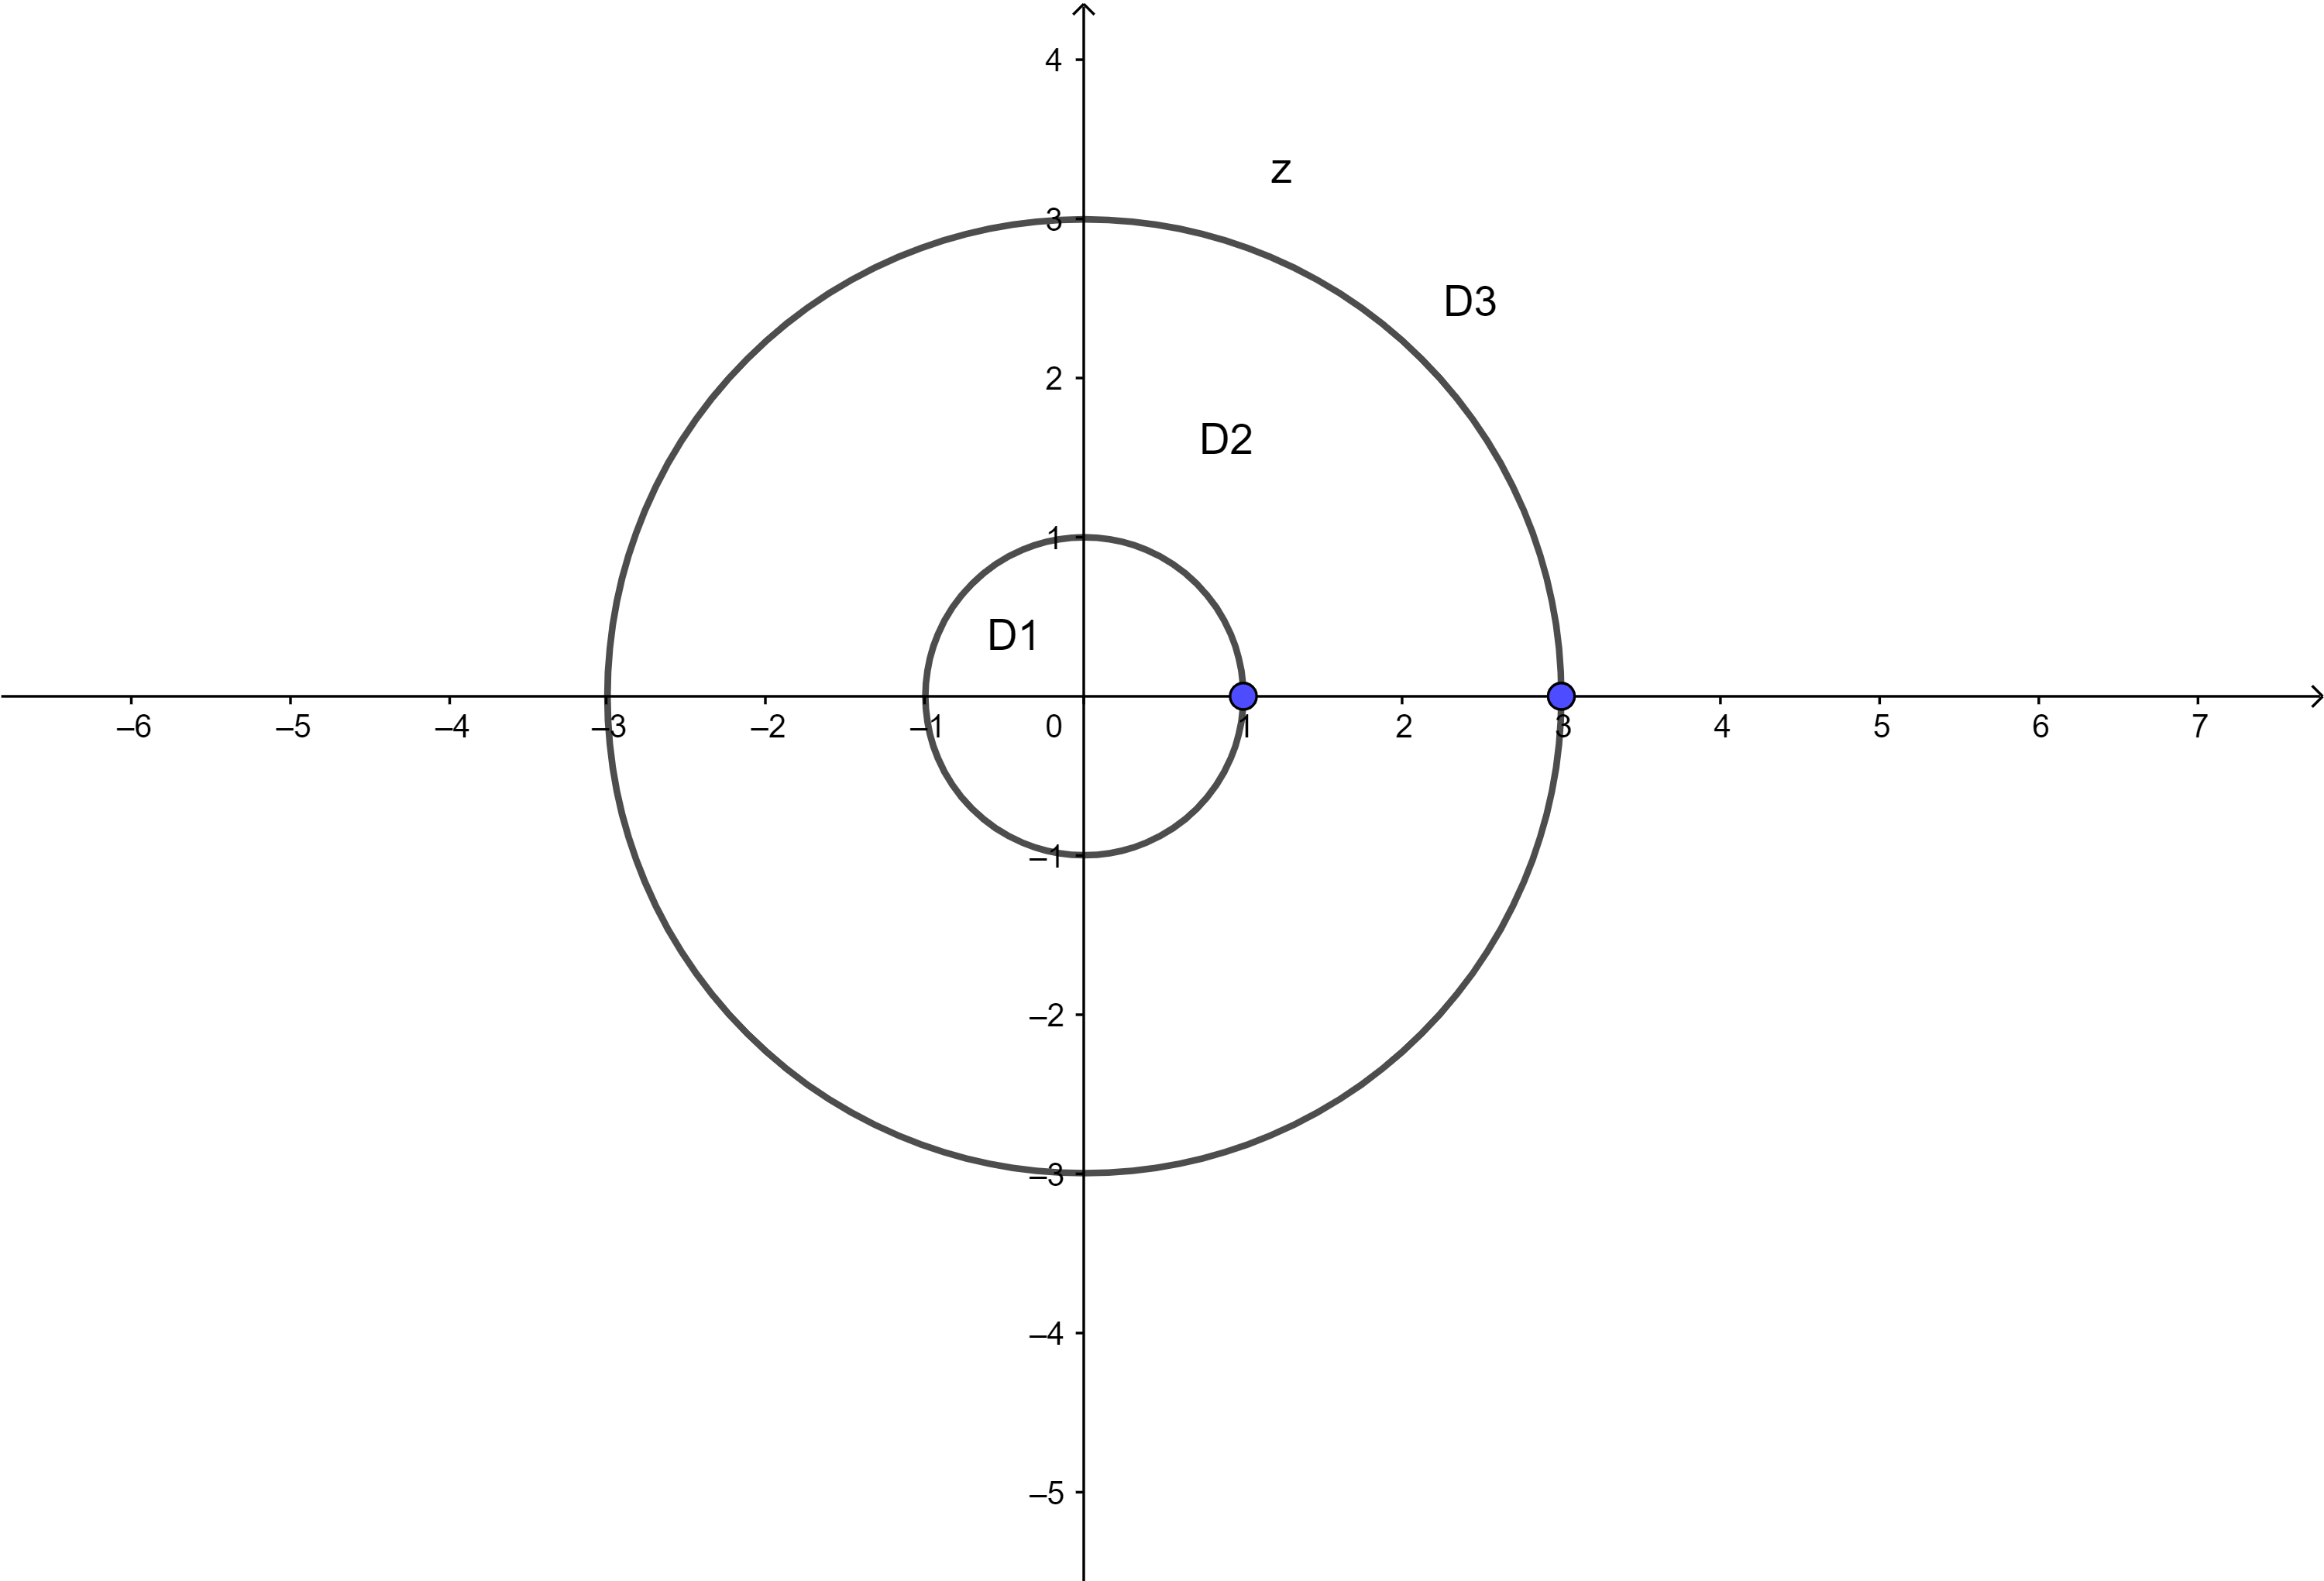
\includegraphics[scale = 0.85]{lec34_1} 
		\end{center}
		
		\begin{enumerate}
			\item В $ D_1 $ $ f(z) $ аналитична, поэтому здесь ряд Лорана дает 
			соответствующий СтР относительно $ z > 0 $:
			\[ f(z) = \frac{z + 1}{(z + 1)(z - 3)} = \frac{1}{z - 3} = 
			-\frac{\frac{1}{3}}{1 - \frac{z}{3}} = \left[
			\begin{array}{l}
			z \in D_1 \implies |z| < 1\\
			q = \frac{z}{3},\ |q| < 1
			\end{array}
			\right] = \]
			\[ = -\frac{1}{3} \sum\limits_{n = 0}^{\infty} \frac{z^n}{3^n}. \]
			
			\item $ z \in D_2 $. Здесь будет та же логика, что и в (а), так как $ -1 $ 
			~--- устранимая особая точка.
			
			\item $ z \in D_3 $. Здесь будет отличие только в степени $z$:
			
			\[ f(z) = \frac{1}{z(1 - \frac{3}{z})} = \left[ |z| > 3,\ |q| = 
			\left|\frac{3}{z}\right| < 1 \right] = \frac{1}{z} \sum\limits_{n = 
			0}^{\infty} 
			\frac{3^n}{z^n} = \sum\limits_{n = 0}^{\infty} \frac{3^n}{z^{n + 1}}. \]
		\end{enumerate}
	
		\item \[ f(z) = \frac{z}{(z + 1)(z - 2)},\ 1 < |z| < 2 \]
		
		В этом случае рассматриваем только область $ D_1 $.
		\begin{center}
			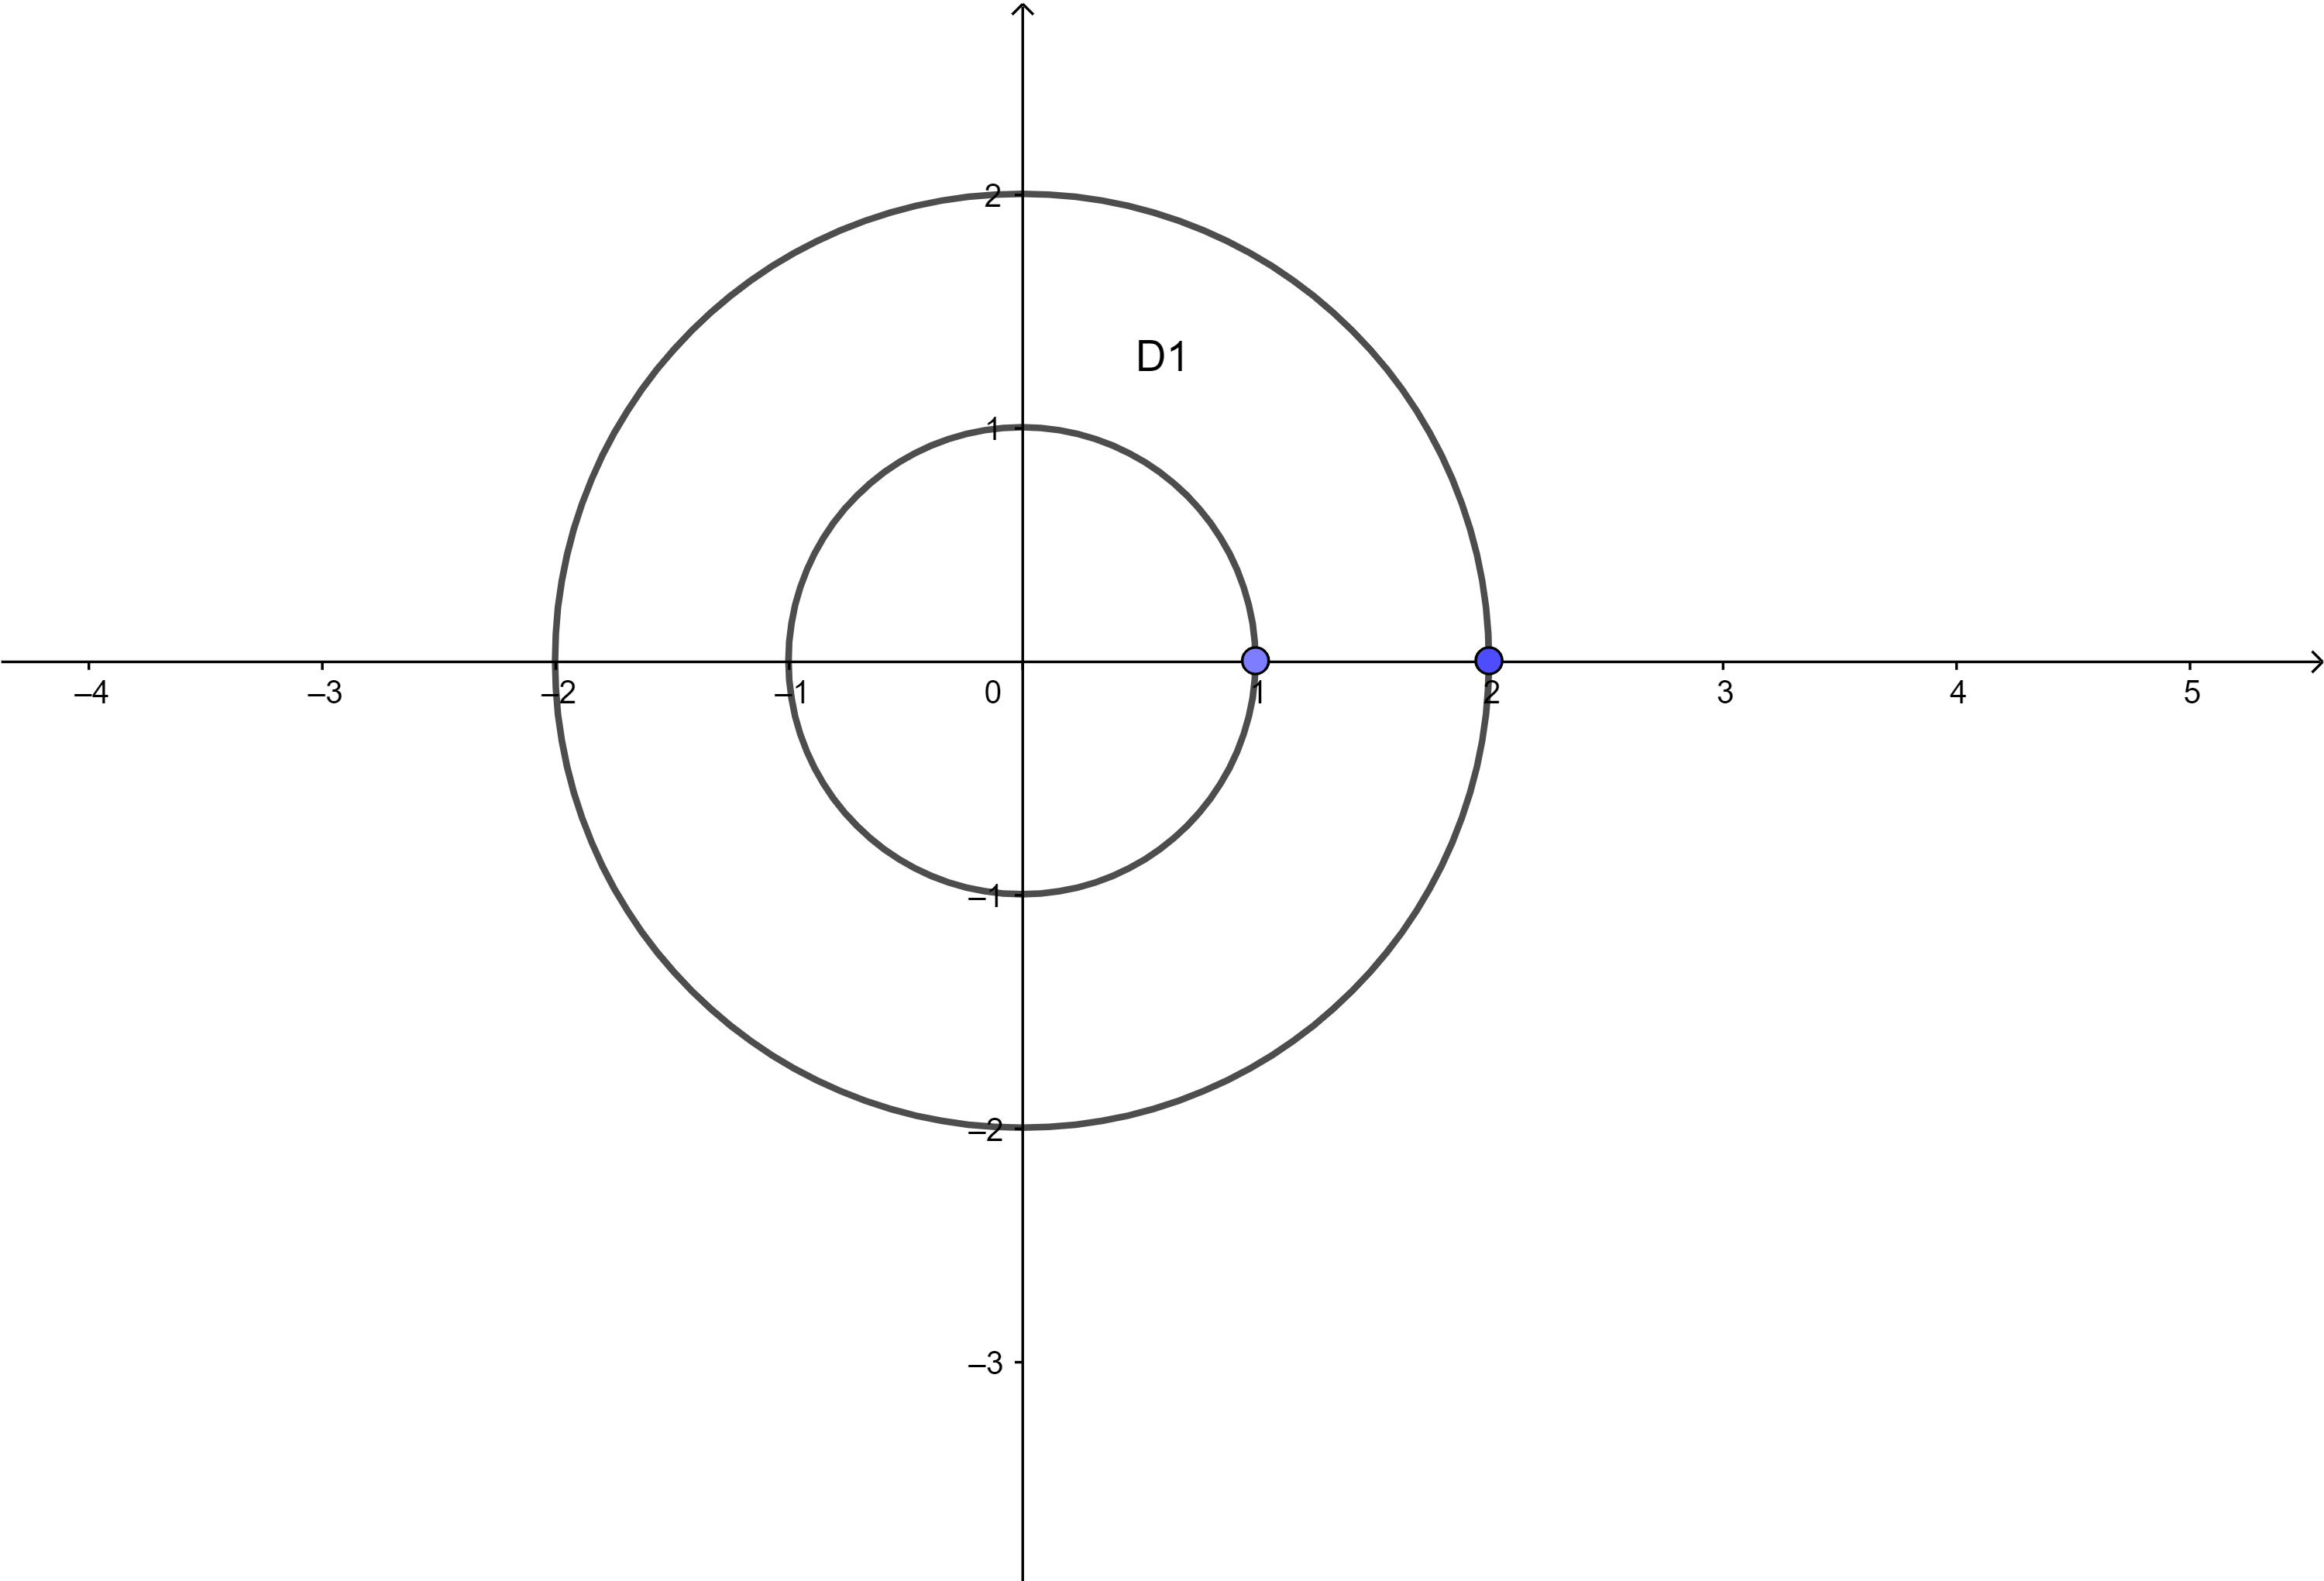
\includegraphics[scale = 1]{lec34_2} 
		\end{center}
	
		Разлагая функцию $ f(z) $ на простые, имеем:
		\[ f(z) = \frac{1}{3(1 + z)} + \frac{2}{3(z - 2)} = \frac{1}{3z(1 + 
		\frac{1}{z})} - \frac{1}{3(1 - \frac{z}{2})} = \left[ 
		\left|\frac{1}{z}\right| < 1,\ 
		\left|\frac{z}{2}\right| < 1 \right] = \]
		\[ = \frac{1}{3z} \sum\limits_{n = 0}^{\infty} \frac{(-1)^n}{z^n} - 
		\frac{1}{3} \sum\limits_{n = 0}^{\infty} \frac{z^n}{2^n} = \frac{1}{3} 
		\left( -\sum\limits_{n = 0}^{\infty} \frac{z^n}{2^n} + \sum\limits_{n = 
		0}^{\infty} \frac{(-1)^n}{z^{n + 1}} \right). \]
	\end{enumerate}
\end{exmps}
\end{document}
